\documentclass{article}
\usepackage{amsmath}
\usepackage{graphics}
\usepackage{hyperref}
\usepackage[pdftex]{graphicx} % with the driver option
\title{The hybrid ray tracer}
\author{Arthur Adriaens}
\date{\today}

\begin{document}
	\maketitle
	\section{random number generator}
	We'll use the numpy random module to generate the random numbers, the considered square (as there is only a z component to the ice model the 3D problem is essentially only a 2D problem) is x:-4km,+4km and z:0,-3km. A good test to see if the generator is both random and uniform is to plot the next element to the previous element, here shown for the generated z coordinates,
\begin{figure}[ht]
	\centering
	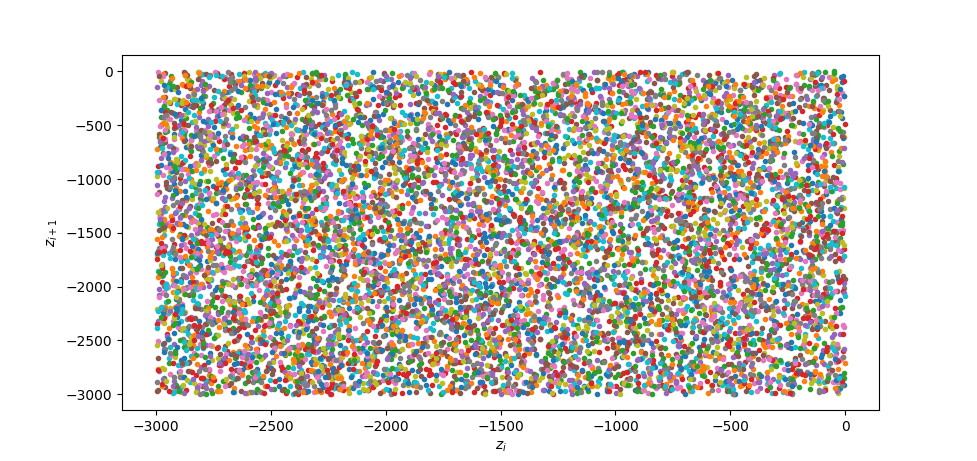
\includegraphics[width=0.8\textwidth]{figures/randomnumberz.png}

\end{figure}
,for the generated x coordinates,
\begin{figure}[ht]
	\centering
	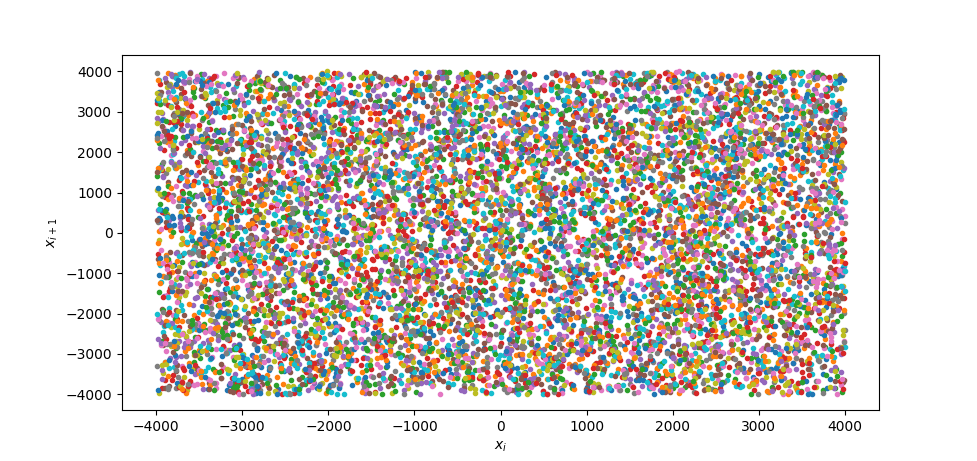
\includegraphics[width=0.8\textwidth]{figures/randomnumberx.png}
\end{figure}
and for the cross of the two.
\begin{figure}[ht]
	\centering
	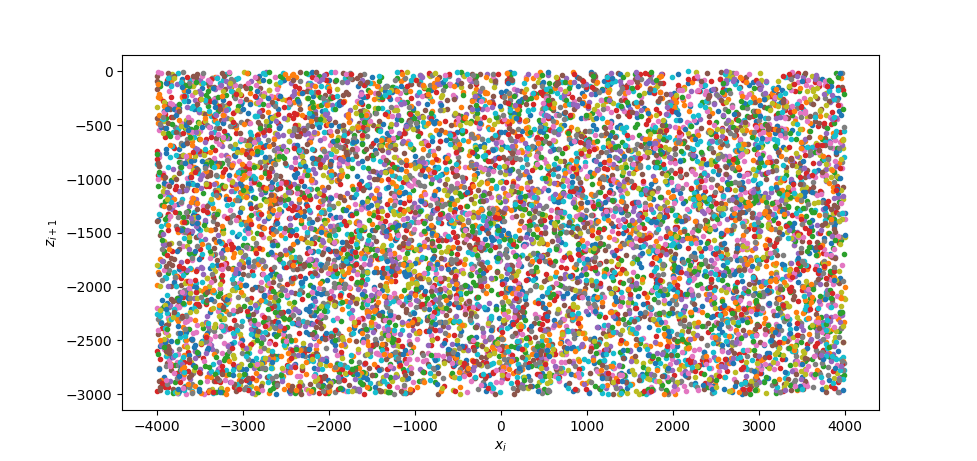
\includegraphics[width=0.8\textwidth]{figures/randomnumbercross.png}
\end{figure}
This clearly is a good random number generator and is the one we'll be using for the testing of the hybrid ray tracer. 
As a counter-example, here is what a bad random number generator would look like
\begin{figure}
	\centering
	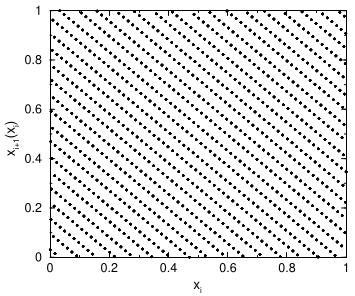
\includegraphics[width=0.5\textwidth]{figures/BadRandom.png}
	\caption{bad random number generator}
\end{figure}
average minimizer time is 1.1645308179855347 seconds
average iterative time is 1.7735618104934692 seconds
\end{document}
